\documentclass{beamer}
\usetheme{default}

\usepackage{etoolbox}
\usepackage{tikz}
\usepackage{xcolor}
\usepackage{multicol}
\usepackage{fontawesome5}
\usepackage{hyperref}
\usepackage{natbib}
\usepackage{subcaption}
\usepackage{booktabs}

\definecolor{alpha}{RGB}{0, 91, 156}
\definecolor{beta}{RGB}{169, 205, 64}
\definecolor{gamma}{RGB}{4, 178, 226}

\setbeamercolor{title page}{bg=alpha}

% custom footer
\setbeamertemplate{footline}{
    \begin{tikzpicture}[remember picture,overlay]
        \node[anchor=south west, xshift=-0.14cm, yshift=0]
          at (current page.south west) {\centering 
\includegraphics[width=\paperwidth]{figs/icipe_bt_line.png}};
        \node[anchor=south east, xshift=-0.14cm, yshift=0.55cm]
          at (current page.south east) {\centering 
\includegraphics[width=1.2cm]{figs/icipe_logo.png}};
        \node[anchor=south west, xshift=0.01cm, yshift=0.5cm, text width=0.4\paperwidth, inner sep=5pt]
          at (current page.south west){{\tiny www.icipe.org}};
        \node[anchor=south east, xshift=-0.2cm, yshift=0.2cm, font=\tiny, text=black, color=white] at (current page.south east) {\insertframenumber};
    \end{tikzpicture}
}

% custom header
\setbeamertemplate{headline}{
    \begin{beamercolorbox}[wd=\paperwidth,ht=0.7cm,dp=0.2cm]{headline}
        
\begin{tikzpicture}
            \fill[left color=gamma, right color=alpha] (0,0) rectangle (\paperwidth,0.5cm);
            \node[anchor=east, xshift=-0.5cm, text=white, font={\bfseries\small}] at (\paperwidth, 0.25cm) {\insertsection};
        \end{tikzpicture}
        \begin{columns}[T,onlytextwidth]
            \column{0.48\textwidth}
            \raggedright\insertsectionnavigationhorizontal{\textwidth}{\hskip0pt plus1fill}{\hskip0pt plus1fill}
            \column{0.48\textwidth}
            \raggedleft\insertsubsectionnavigationhorizontal{\textwidth}{\hskip0pt plus1fill}{\hskip0pt plus1fill}
        \end{columns}
    \end{beamercolorbox}
}

\setbeamertemplate{background canvas}{
    \begin{tikzpicture}
        \fill[white] (current page.south west) rectangle (current page.north east);
    \end{tikzpicture}
}

\title{Bridging Critical Data Gaps in Vector-Borne Disease Surveillance:\\
A Reproducible Computational Framework Integrating Heterogeneous Data through a Common Data Model}
\author{Salvador D. ATAGONG}
\date{\today}

\begin{document}

% title page
\begin{frame}[noframenumbering, plain]
    \begin{tikzpicture}[remember picture,overlay]
        \fill[alpha] (current page.south west) rectangle (current page.north east);
        \node[anchor=south, text width=0.8\paperwidth, align=center, font=\bfseries\Large, text=white]
          at ([yshift=1.5cm]current page.center) {{\fontsize{14pt}{16.8pt}\selectfont \inserttitle}};
        \node[anchor=north, yshift=-0.01cm, text width=0.8\paperwidth, align=center, font=\normalfont\large, text=white]
          at ([yshift=1.1cm]current page.center) {\insertauthor};
        \node[anchor=north, yshift=-0.5cm, text width=0.8\paperwidth, align=center, font=\normalfont\large, text=white]
          at ([yshift=0.5cm] current page.center) {\insertdate};
        \node[anchor=north west, xshift=-0.14cm, yshift=-0.5\paperwidth,]
          at (current page.north west) {\centering 
\includegraphics[width=\paperwidth]{figs/icipe_cover_insects.png}};
        \node[anchor=north west, xshift=0, yshift=-0.625\paperwidth,
        fill=white, minimum height=2cm, text width=\paperwidth, inner sep=5pt]
        at (current page.north west){}; 
        \node[anchor=north east, xshift=-0.14cm, yshift=-0.64\paperwidth,]
          at (current page.north east) {\centering 
\includegraphics[width=2.5cm]{figs/icipe_logo.png}};
        \node[anchor=north west, xshift=0, yshift=-0.66\paperwidth, text width=0.4\paperwidth, inner sep=5pt]
        at (current page.north west){www.icipe.org};
    \end{tikzpicture}
\end{frame}

% outline
\begin{frame}
    \frametitle{Outline}
    \begin{multicols}{2}
        \tableofcontents
    \end{multicols}
\end{frame}

\section{Context \& Problem}
\begin{frame}
    \frametitle{Vector-Borne Diseases: A Persistent Challenge}
    \begin{figure}
        \centering
        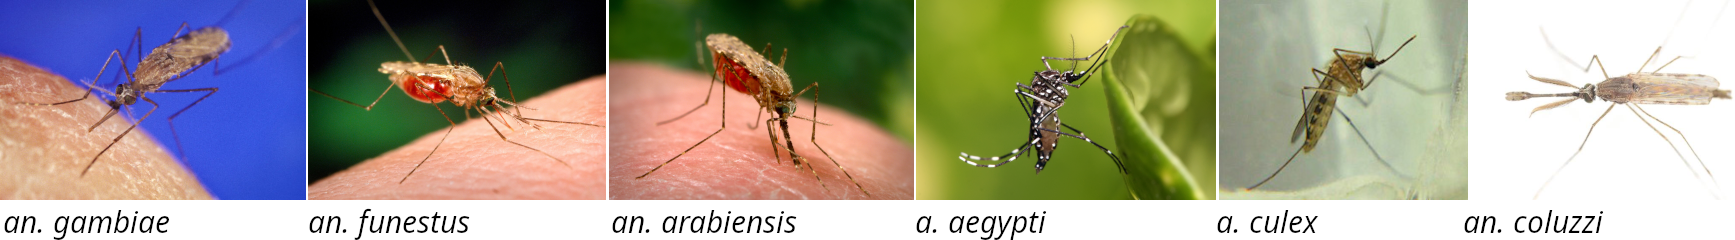
\includegraphics[width=0.7\paperwidth]{figs/list_of_vectors.png}
    \end{figure}
    \begin{itemize}
        \item \textbf{700,000} deaths annually (WHO) - mostly in sub-Saharan Africa.
        \item Malaria alone: \textbf{249M cases}, \textbf{608k deaths} per year.
        \item Emerging threats: invasive \textit{Anopheles stephensi} in urban Africa.
        \item \textbf{Critical data gaps} hinder surveillance, modeling, and control.
    \end{itemize}
\end{frame}

\begin{frame}
    \frametitle{The Data Gap Challenge}
    \begin{itemize}
        \item Vast amounts of VBD data are \textbf{unstructured} (PDFs, figures) - 85\% of all data.
        \item \textbf{Fragmented sources}: GBIF, Vector Atlas, ERA5-Land, Malaria Atlas Project, etc.
        \item \textbf{No standardization} across entomological, climatic, socio-economic data.
        \item Manual extraction takes \textbf{15-30 minutes per document} $\rightarrow$ not scalable.
        \item Result: \textbf{Delayed} decisions, \textbf{ineffective} interventions, \textbf{uninformed} policies.
    \end{itemize}
    \vspace{0.3cm}
    \centering
    \textcolor{alpha}{\textbf{Need for an integrated, reproducible, and scalable framework.}}
\end{frame}

\section{Research Questions \& Hypotheses}
\begin{frame}
    \frametitle{Research Questions}
    \begin{enumerate}
        \item Can a \textbf{Common Data Model (CDM)} harmonize heterogeneous VBD data (occurrence, bionomics, climate, socio-economics) to enable reproducible spatio-temporal analysis?
        \item How do \textbf{Large Language Models (LLMs)} compare to manual extraction in speed and accuracy for mining vector data from scientific literature?
        \item Can a \textbf{multi-agent simulation (MAS)} framework synthesize missing surveillance data and identify environmental tipping points for invasive vectors?
    \end{enumerate}
\end{frame}

\begin{frame}
    \frametitle{Hypotheses}
    \begin{itemize}
        \item \textbf{H1}: A CDM-based integration significantly improves the consistency and reusability of VBD data across sources.
        \item \textbf{H2}: LLM-based extraction reduces document processing time from minutes to seconds while maintaining biological plausibility and scalability.
        \item \textbf{H3}: MAS can generate biologically grounded synthetic data that reveal vector persistence mechanisms in data-scarce urban environments.
    \end{itemize}
\end{frame}

\section{Objectives \& Approach}
\begin{frame}
    \frametitle{Overall Objective}
    \centering
    \large
    \textbf{To develop a reproducible computational framework that bridges critical data gaps in VBD surveillance by integrating heterogeneous environmental and epidemiological data through a specialized Common Data Model (CDM).}
\end{frame}

\begin{frame}
    \frametitle{Three Interlocking Components (1/2)}
    \begin{columns}[T]
        \begin{column}{0.2\textwidth}
            \centering
            \includegraphics[width=0.9\linewidth]{figs/aie_concept.png}\\
            \small
            \textbf{Manuscript 1}\\
            LLM-based data extraction
        \end{column}
        \begin{column}{0.4\textwidth}
            \centering
            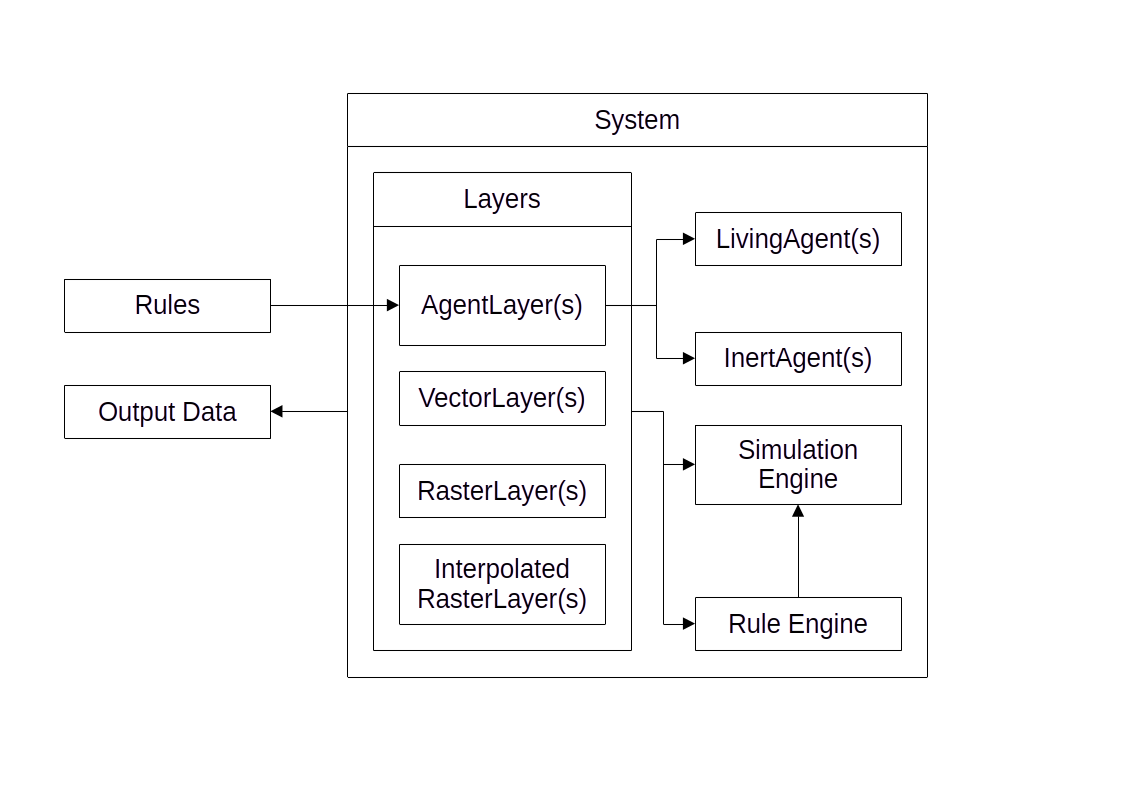
\includegraphics[width=0.9\linewidth]{figs/rmas_architecture.png}\\
            \small
            \textbf{Manuscript 2}\\
            Multi-agent simulation
        \end{column}
        \begin{column}{0.3\textwidth}
            \centering
            
\includegraphics[width=0.9\linewidth]{figs/cdm_concept.png}\\
            \small
            \textbf{Manuscript 3}\\
            Common Data Model (CDM)
        \end{column}
    \end{columns}
\end{frame}
% \begin{frame}
%     \frametitle{Three Interlocking Components (2/2)}
%     \begin{itemize}
%         \item \textbf{Feed into} the CDM $\rightarrow$ standardized analytics-ready data.
%         \item \textbf{Validate} via case studies (Anopheles funestus, An. stephensi, Greater Accra).
%     \end{itemize}
% \end{frame}

\section{Manuscript 1: LLM-Based Data Abstraction}
\begin{frame}
    \frametitle{Automated Data Extraction from Literature}
    \begin{itemize}
        \item Pipeline: PDF $\rightarrow$ text extraction (PyPDF + Tesseract OCR) $\rightarrow$ LLM (Gemini 2.5) $\rightarrow$ knowledge triples $\rightarrow$ alignment $\rightarrow$ CSV.
        \item \textbf{Case study}: \textit{Anopheles funestus} in Africa (394 publications, 2003-2025).
        \item \textbf{Results}:
        \begin{itemize}
            \item 129 unique occurrence points extracted.
            \item \textbf{15 seconds per document} (vs. 15-30 min manual).
            \item Centroid distance to manually curated Vector Atlas data: \textbf{572 km} (negligible at continental scale).
            \item Extracted bionomics: indoor resting (18 studies), indoor biting (44 studies), pyrethroid resistance (28 studies).
        \end{itemize}
        \item \textbf{Tool}: NARRATOR (\url{https://narrator.voidmonad.com/}).
    \end{itemize}
\end{frame}

\begin{frame}
    \frametitle{Validation: Occurrence Maps \& Species Distribution (1/2)}
    \begin{figure}
        \centering
        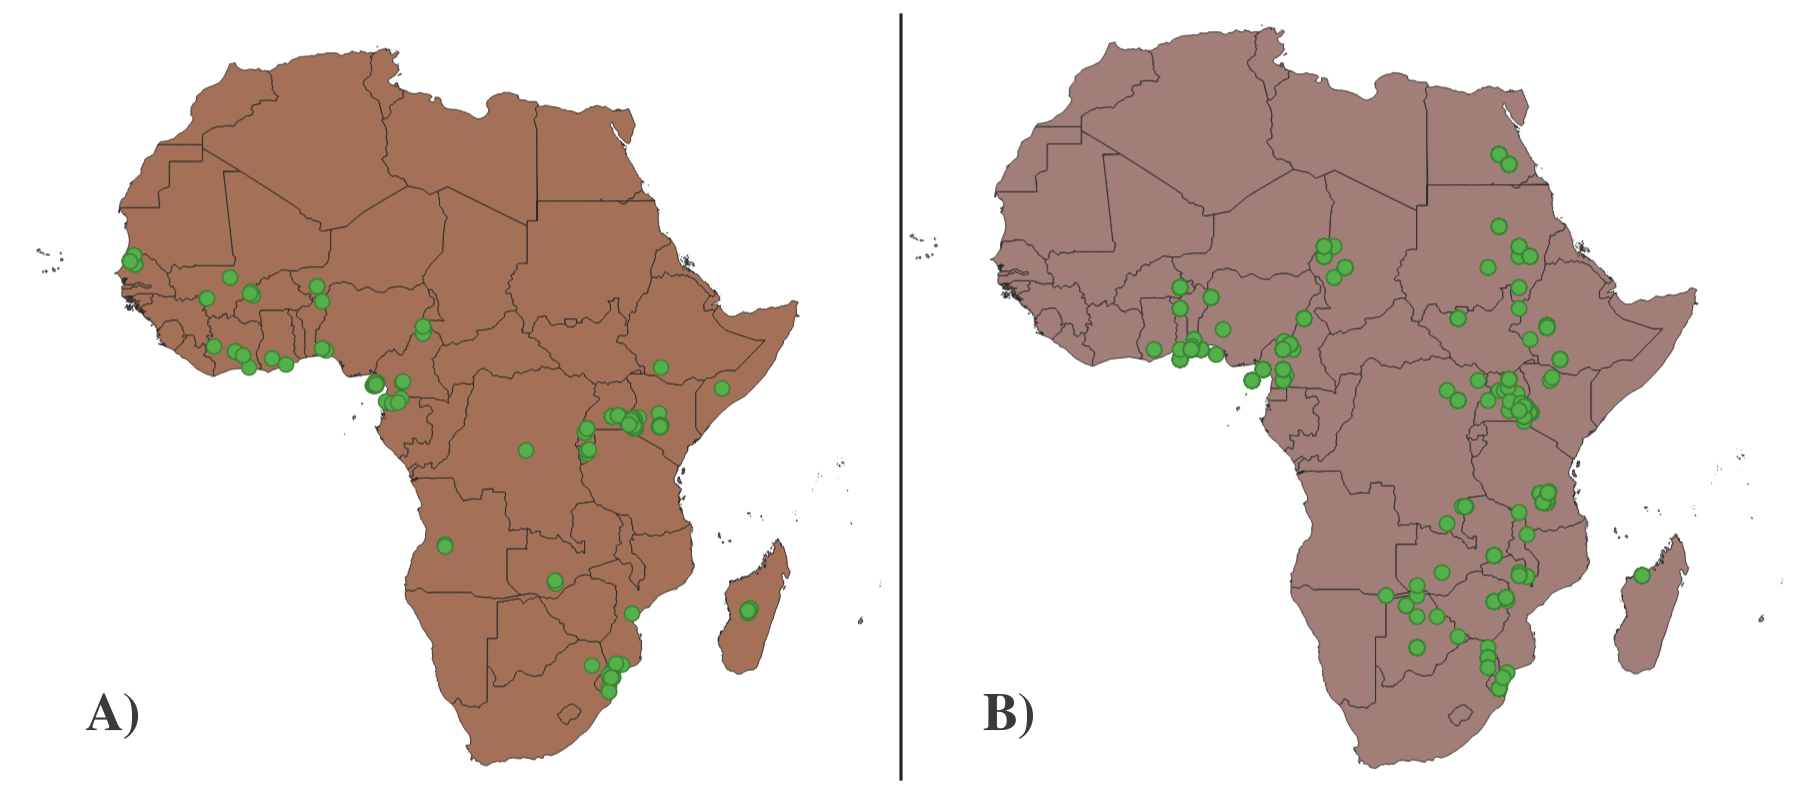
\includegraphics[width=0.8\linewidth]{figs/side_by_side_maps.png}
        \caption{Left: Vector Atlas manual data (315 records). Right: Automatically extracted (129 records).}
    \end{figure}
\end{frame}
\begin{frame}
    \frametitle{Validation: Occurrence Maps \& Species Distribution (2/2)}
    \begin{figure}
        \centering
        \includegraphics[width=0.45\linewidth]{figs/Maxent_Model_Weighted_pd_projection.jpg}
        \caption{MaxEnt habitat suitability for \textit{An. funestus} based on extracted data.}
    \end{figure}
\end{frame}

\section{Manuscript 2: Multi-Agent Simulation}
\begin{frame}
    \frametitle{Synthesizing Missing Surveillance Data}
    \begin{itemize}
        \item \textbf{Problem}: No long-term vector abundance data for invasive \textit{An. stephensi} in urban Africa.
        \item \textbf{Solution}: High-performance rule-based MAS (Java, StampedLock, object pooling).
        \item \textbf{Case study}: Dire Dawa, Ethiopia - 60-day simulation, 5 km radius, 9,805 water containers, 250k+ agents.
        \item \textbf{Performance}: 1.27M rule evaluations/sec, 26.75 ms/tick, total 10 min runtime on standard hardware.
        \item \textbf{Biological output}: Population collapses when temperature exceeds \textbf{37°C}; surviving agents remain within \textbf{45 m} of water infrastructure (refugia).
    \end{itemize}
\end{frame}

\begin{frame}
    \frametitle{System Architecture}
    \begin{figure}
        \centering
        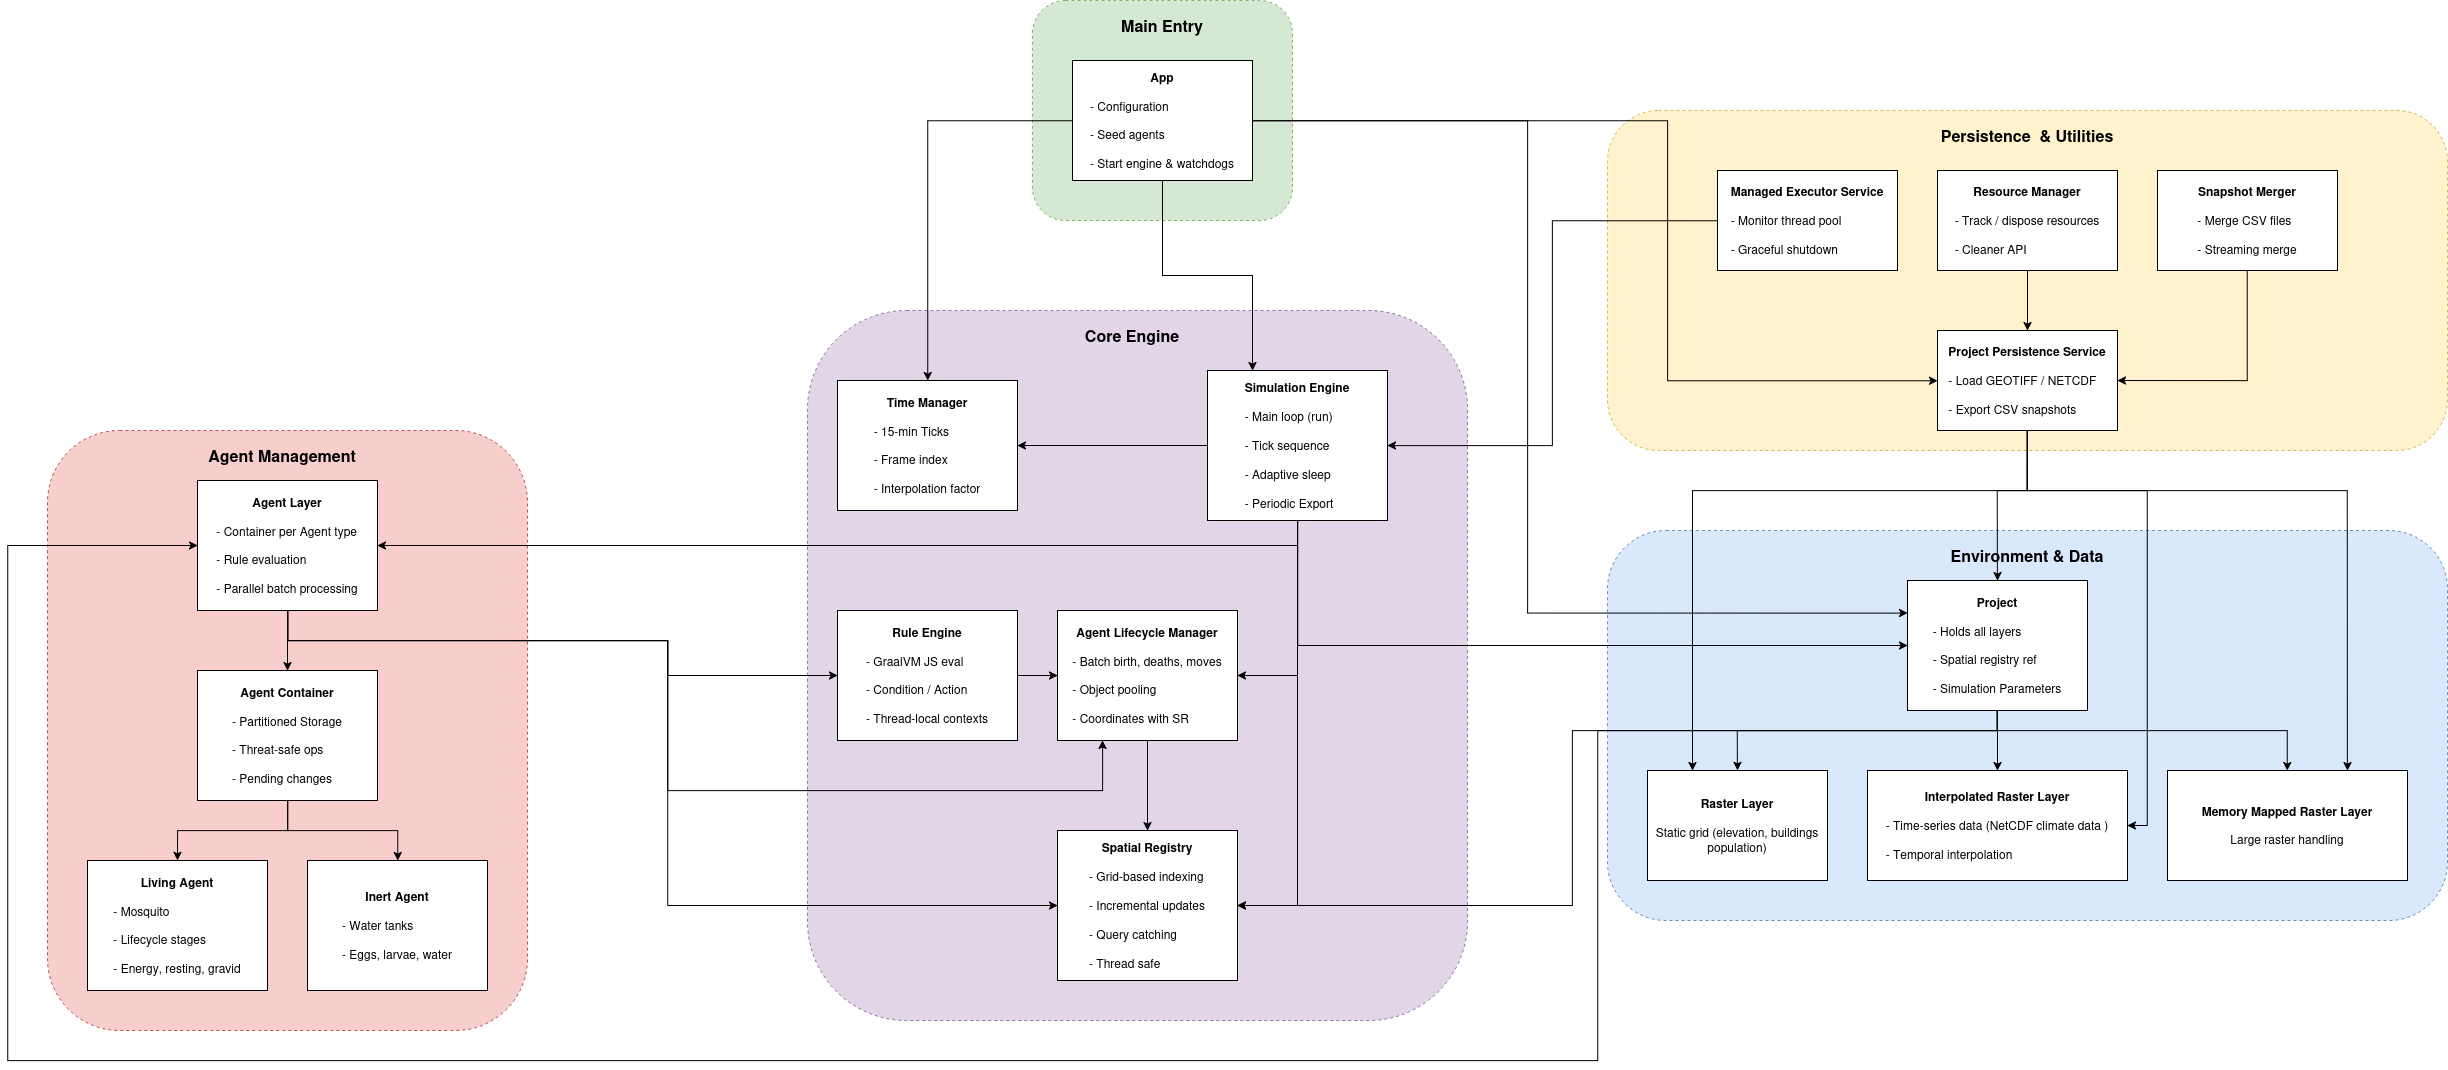
\includegraphics[width=\linewidth]{figs/phd_graphs-rmas.drawio_arch.png}
        \caption{Multi-agent system architecture.}
    \end{figure}
\end{frame}

\begin{frame}
    \frametitle{MAS Results: Tipping Points \& Spatial Clustering}
    \begin{figure}
        \centering
        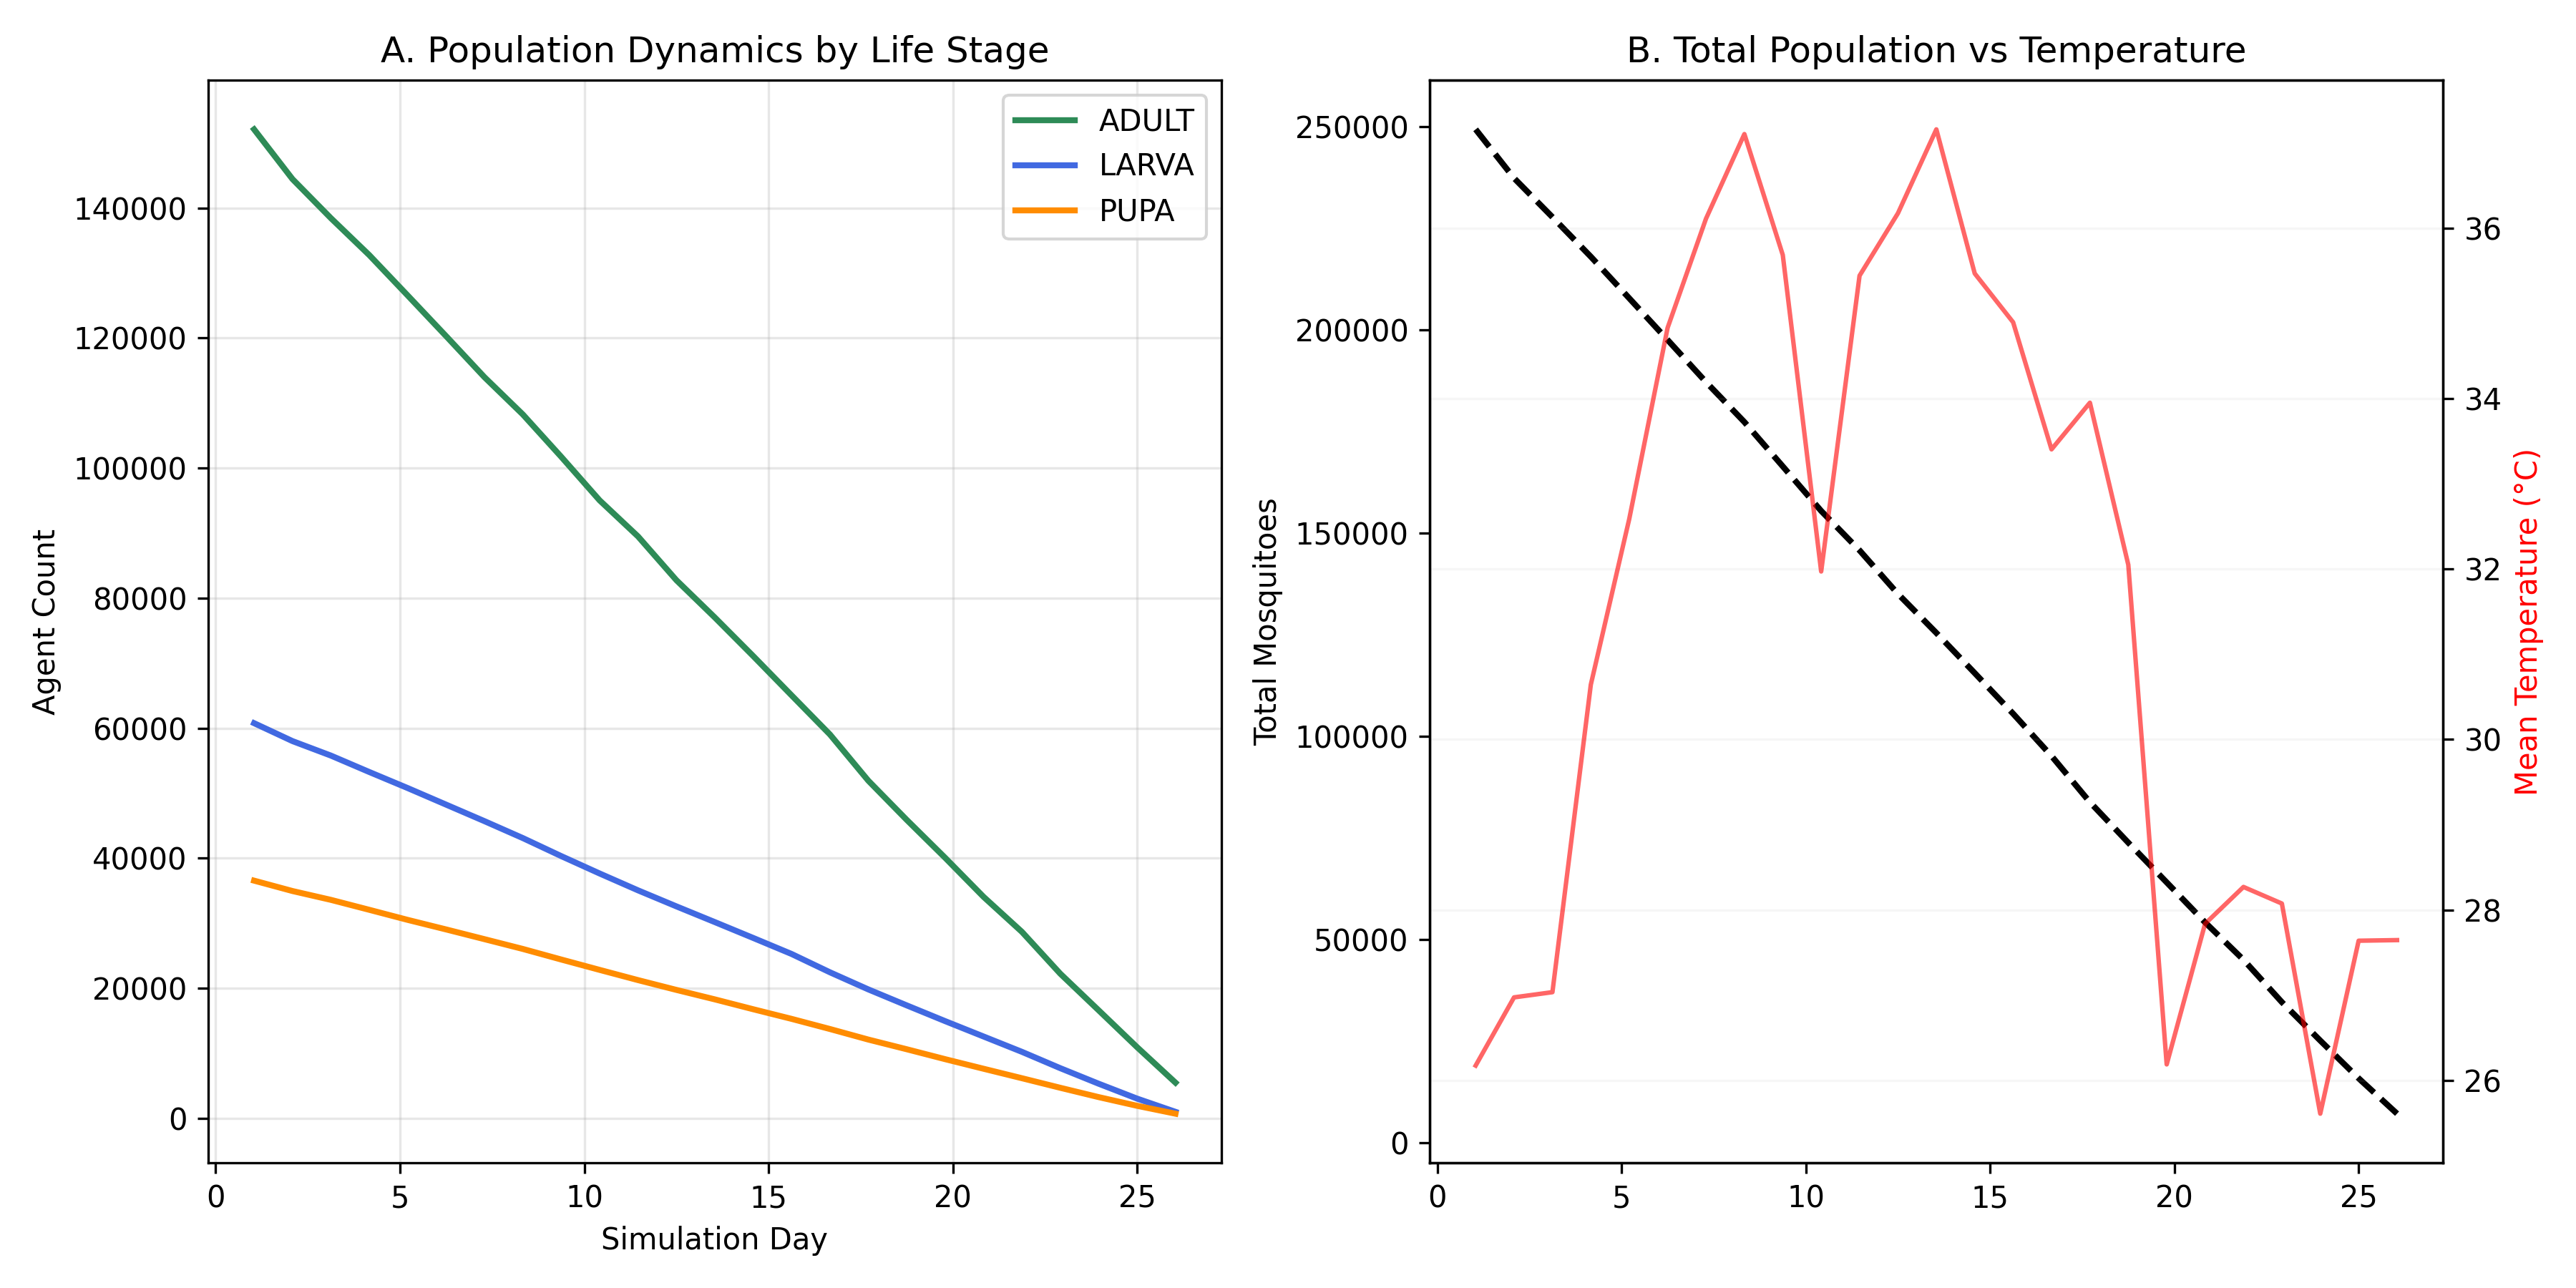
\includegraphics[width=0.45\linewidth]{figs/dynamics_analysis.png}
        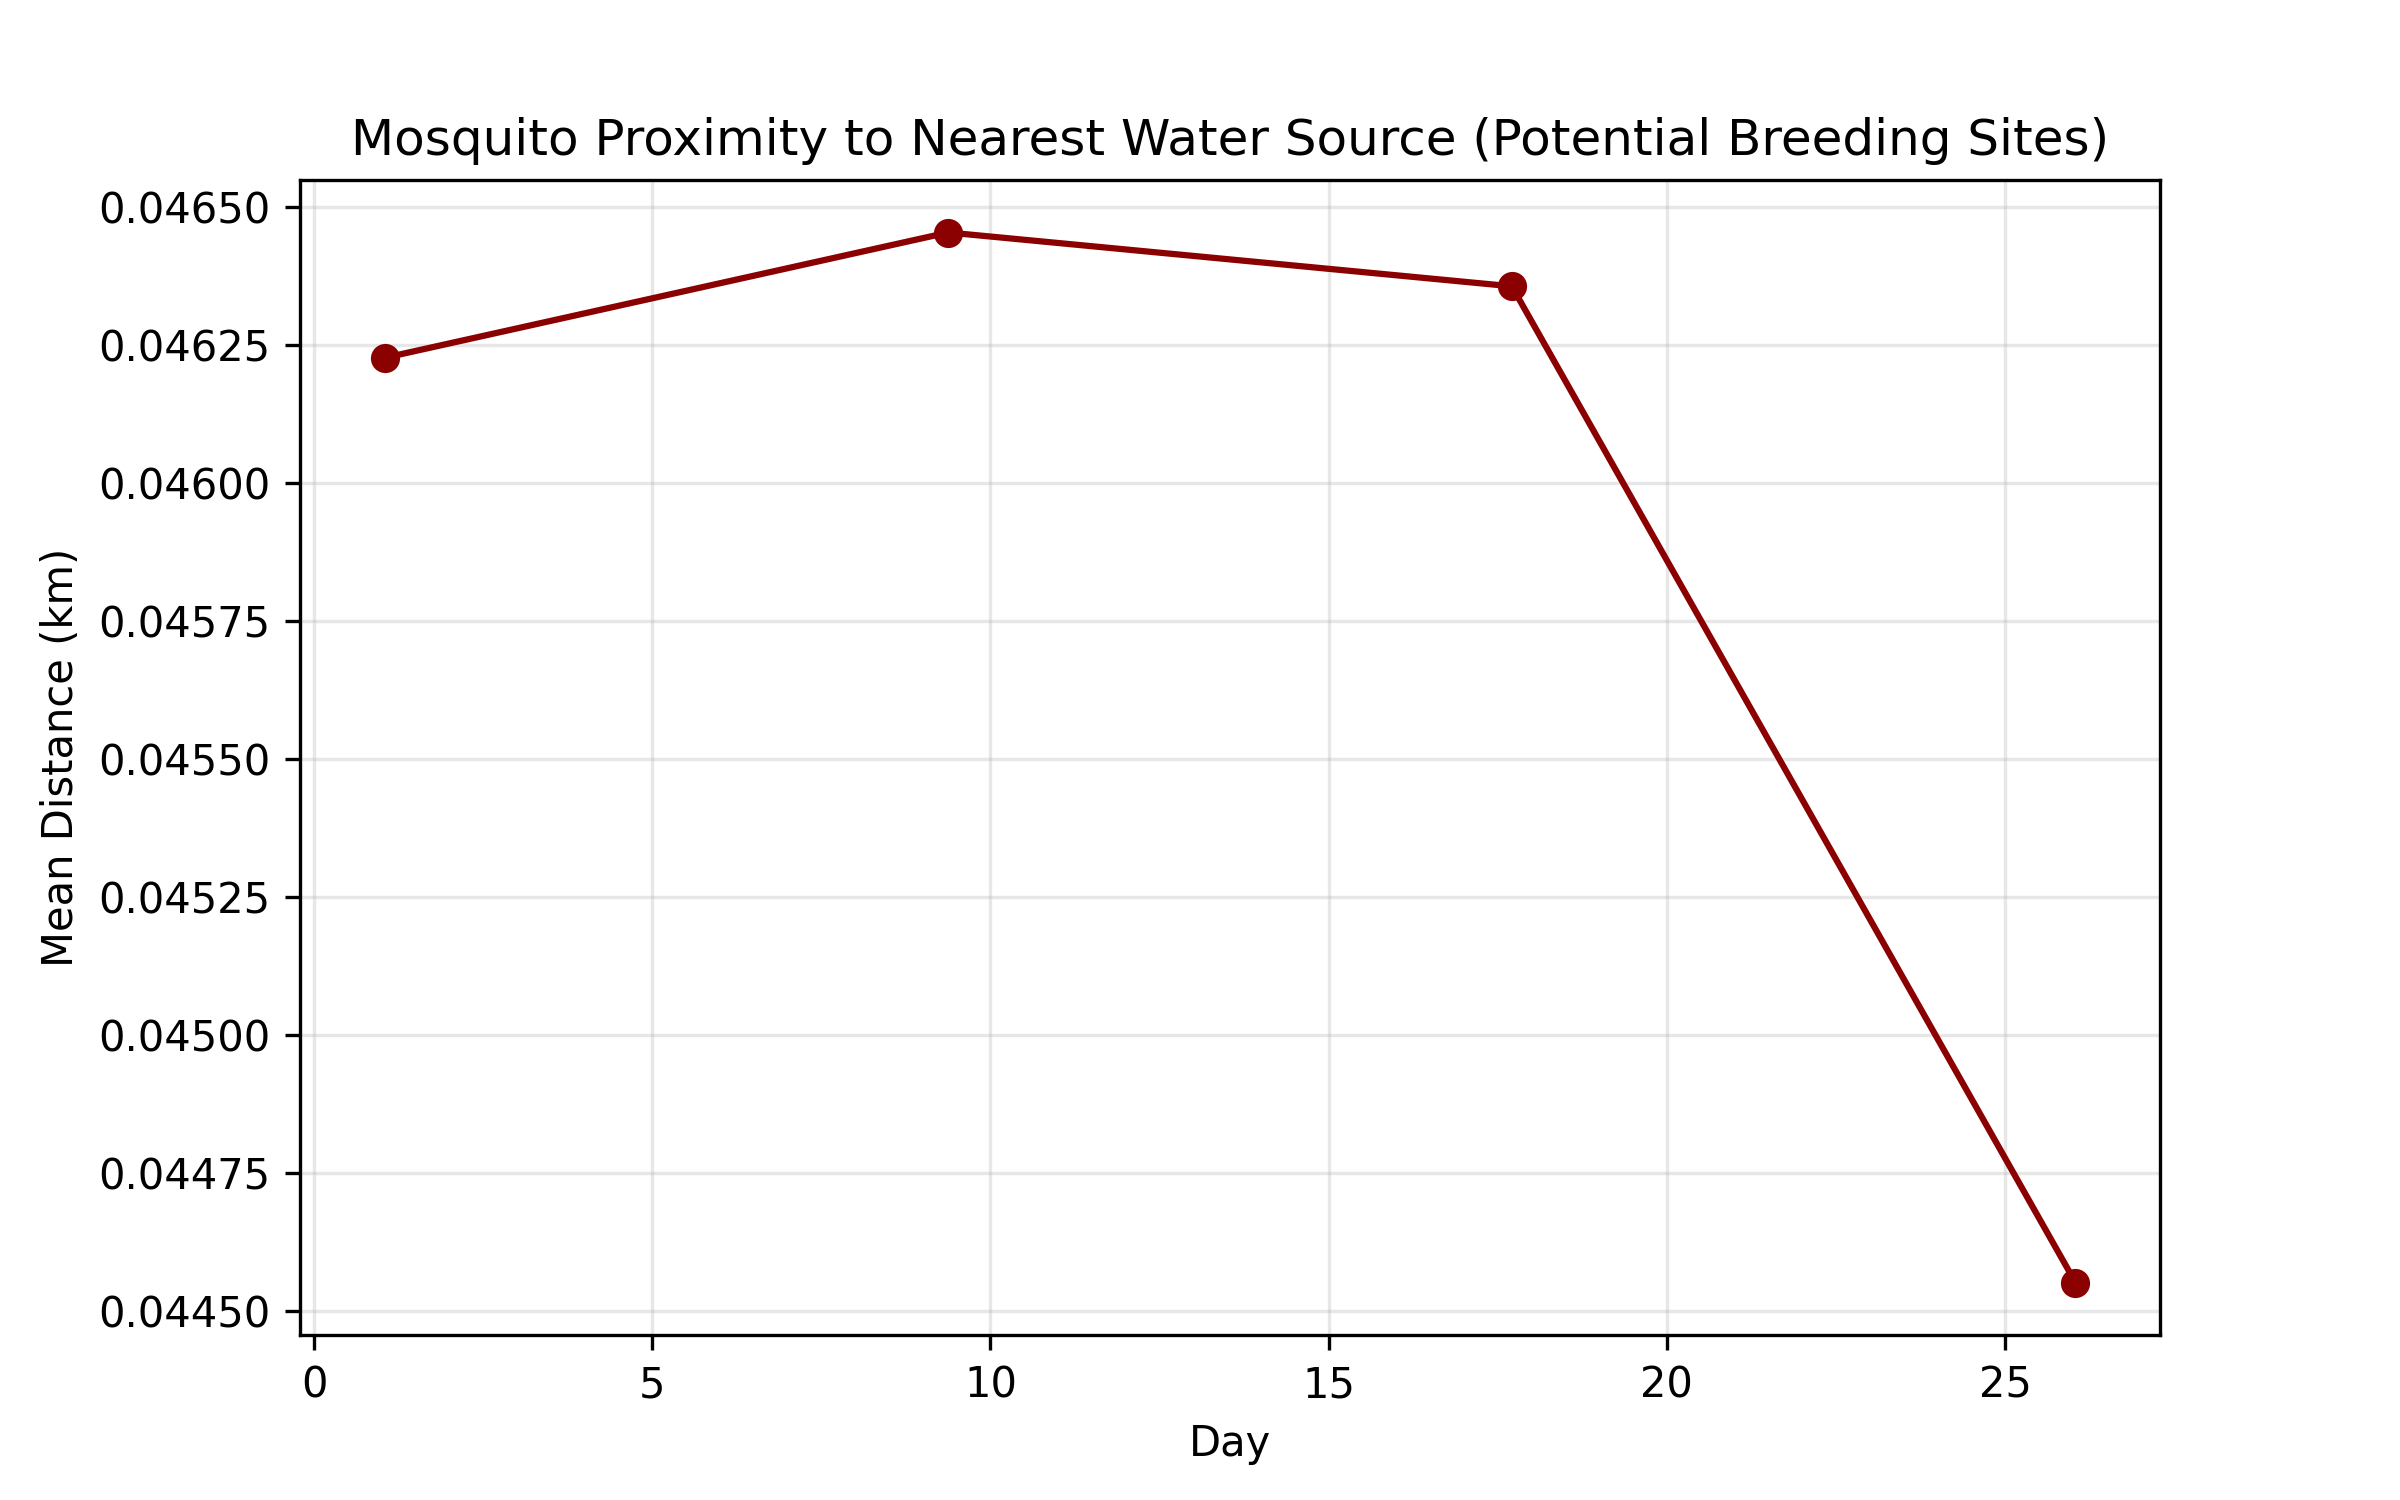
\includegraphics[width=0.45\linewidth]{figs/proximity_trend.png}
        \caption{Population decline above 30°C (left); survivors stay within ~45m of water (right).}
    \end{figure}
    \begin{itemize}
        \item Identifies \textbf{environmental thresholds} for intervention.
        \item Generates \textbf{synthetic data} where field data are absent.
    \end{itemize}
\end{frame}

\begin{frame}
    \frametitle{RMAS refined evaluation approach}
    \begin{multicols}{2}
        \begin{itemize}
            \item Data compilation \& processing
            \item Parameterization \& calibration
            \item Internal validation
            \item Quantitative validation
            \item Sensitivity \& uncertainty analysis
            \item Scenario analysis & Surveillance utility
            \item Reproductibility \& reporting
        \end{itemize}
    \end{multicols}
\end{frame}

\section{Manuscript 3: Common Data Model (CDM)}
\begin{frame}
    \frametitle{CDM Design \& Implementation}
    \begin{columns}[T]
        \begin{column}{0.4\textwidth}
            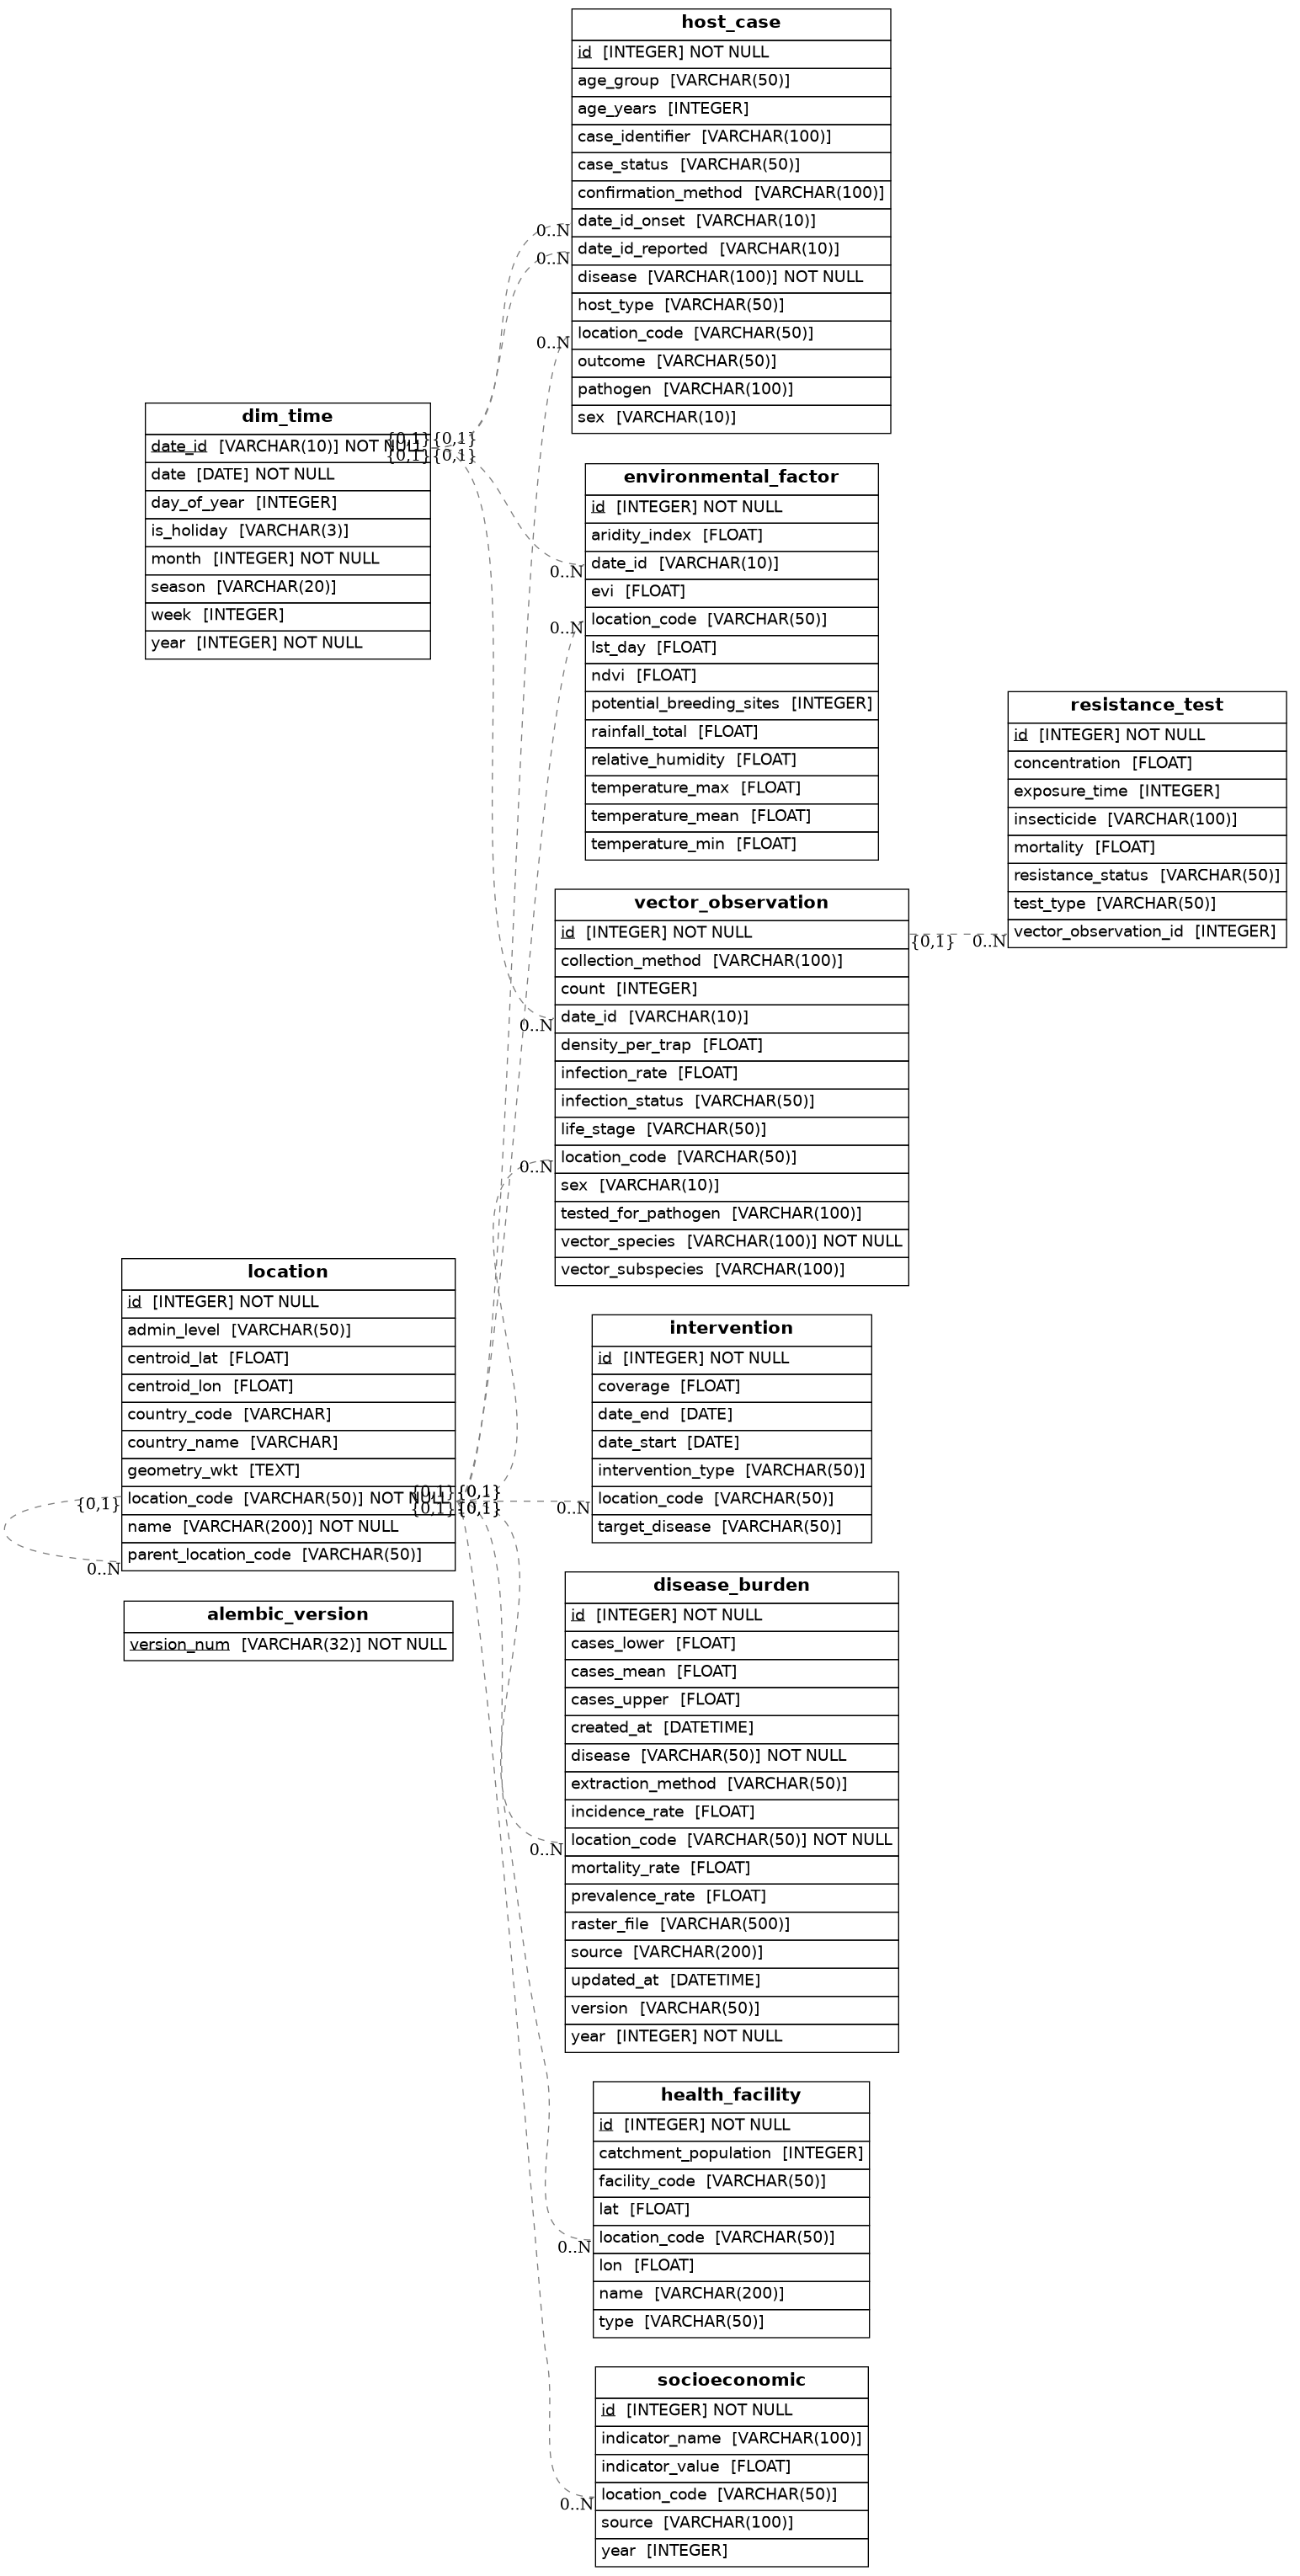
\includegraphics[width=0.75\linewidth,scale=0.05]{figs/er_diagram.png}
        \end{column}
        \begin{column}{0.6\textwidth}
            \small
            \textbf{Star schema} with 8 core tables:
            \begin{itemize}
                \item Dimensions: Time, Location, HealthFacility, Intervention, SocioEconomic
                \item Facts: HostCase, DiseaseBurden, VectorObservation, EnvironmentalFactor, ResistanceTest
            \end{itemize}
            \textbf{Features:}
            \begin{itemize}
                \item Hierarchical locations (country$\rightarrow$region$\rightarrow$district)
                \item Geometry support (WKT)
                \item Metadata tracking (source, version)
            \end{itemize}
        \end{column}
    \end{columns}
\end{frame}

\begin{frame}
    \frametitle{System architecture}
    \begin{figure}
        \centering
        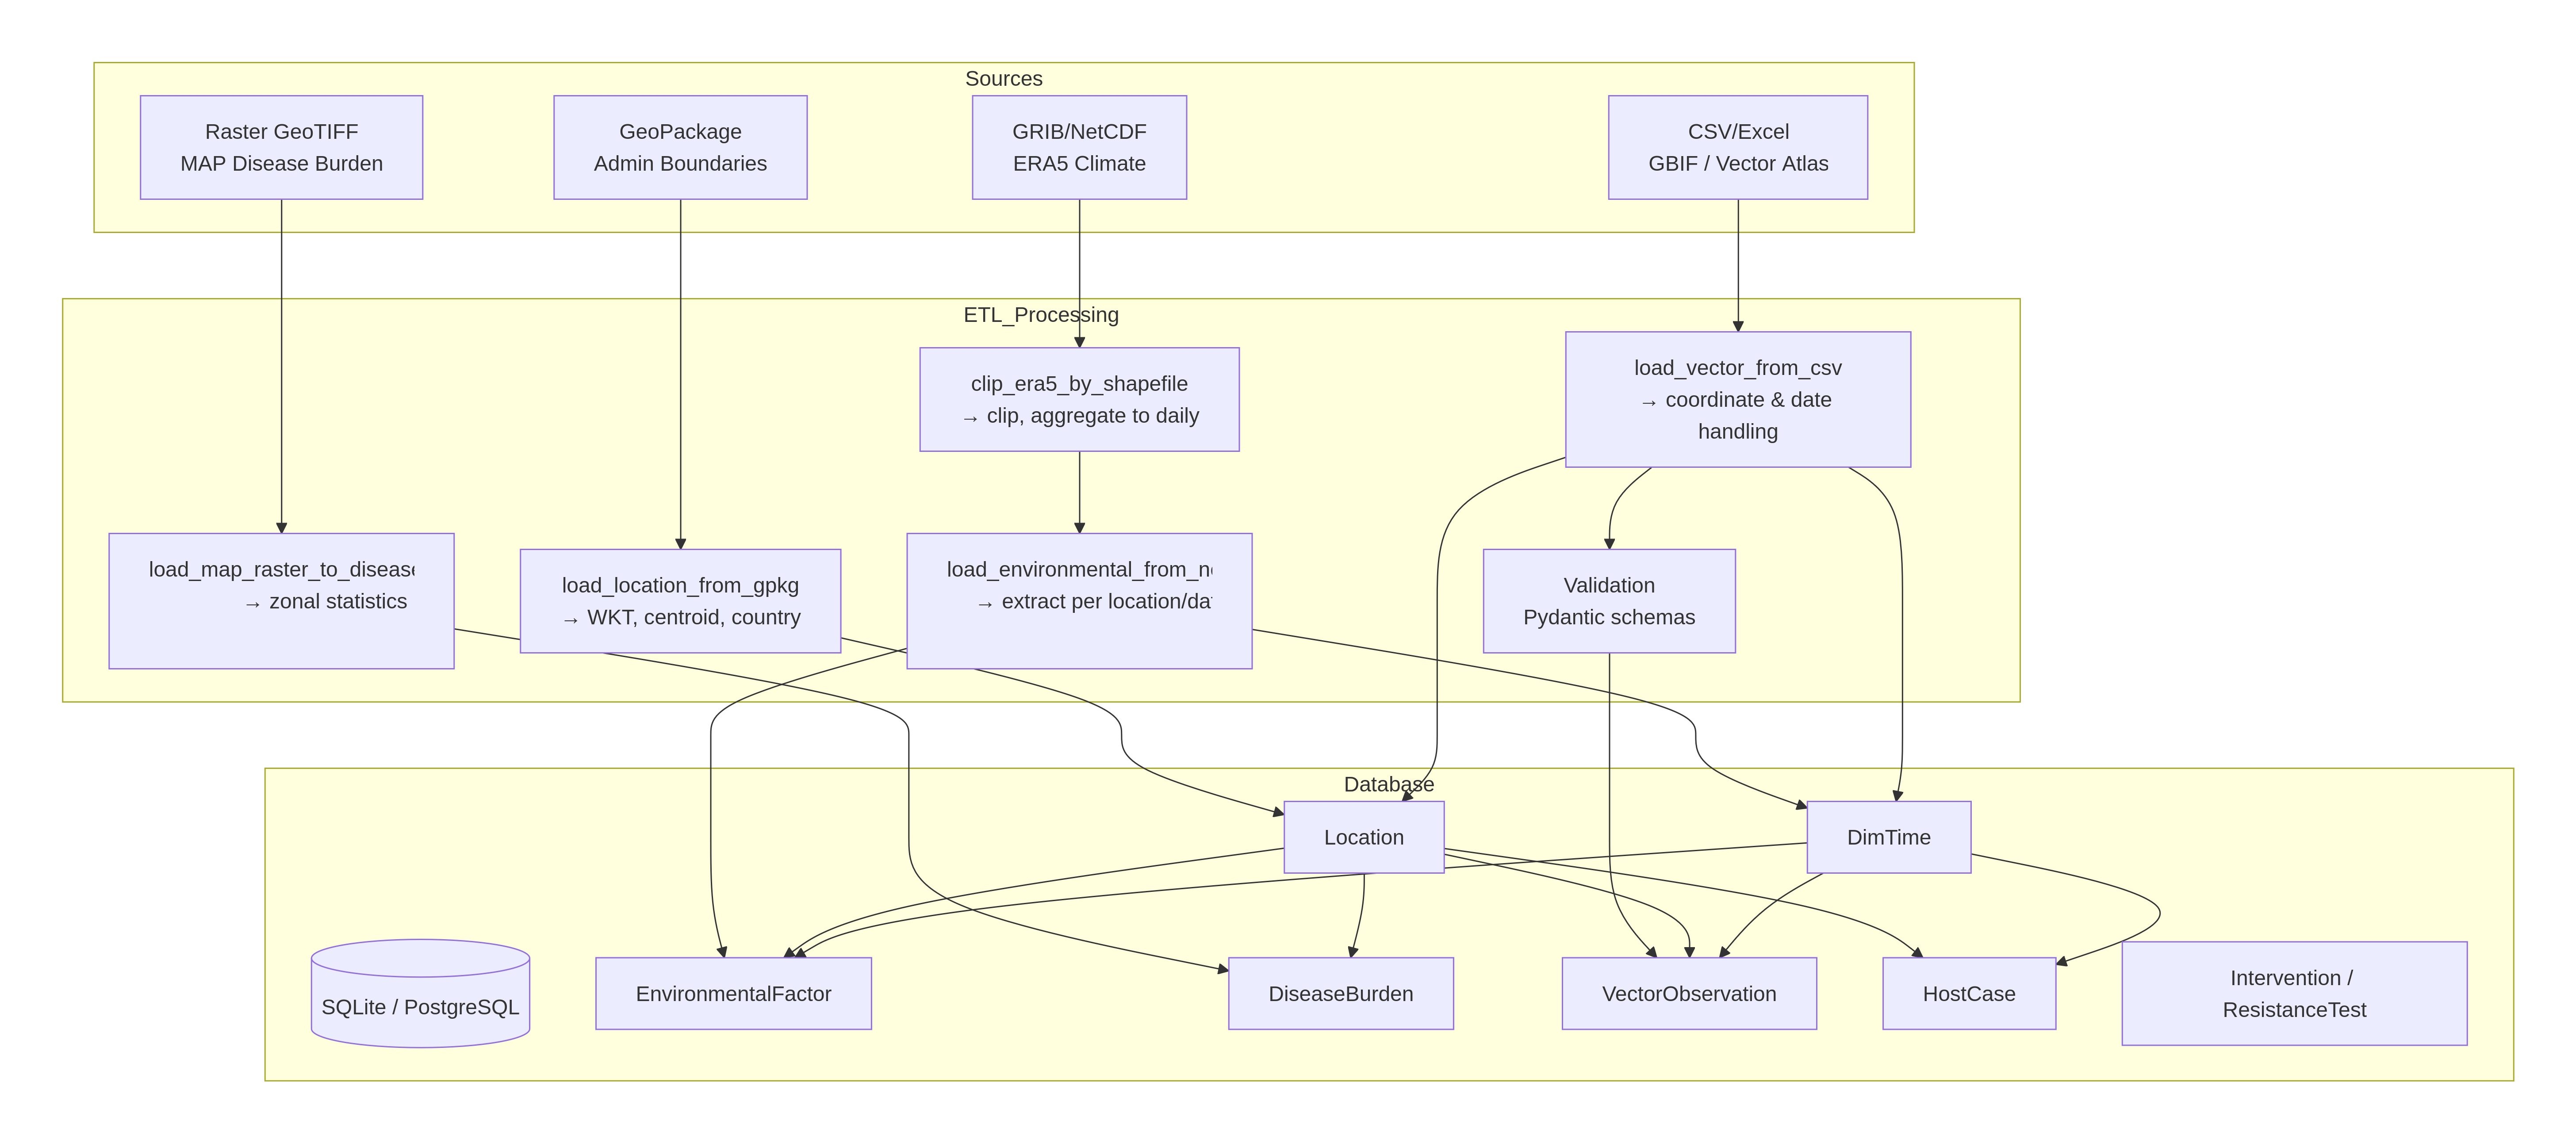
\includegraphics[width=\linewidth]{figs/deepseek_mermaid_vcdm_overview.png}
        \caption{CDM System architecture detailed overview.}
    \end{figure}
\end{frame}

\begin{frame}
    \frametitle{Case Study: Greater Accra, Ghana}
    \begin{itemize}
        \item Integrated GBIF (vector), ERA5-Land (climate), and Malaria Atlas Project (burden).
        \item \textbf{Challenge}: Temporal mismatch - annual burden vs. daily vector/environmental data.
        \item \textbf{Climate-vector analysis} (7 months, Feb 2017-Jun 2018):
        \begin{itemize}
            \item Weak contemporaneous correlations (temp r$\approx$0.11, rain r$\approx$0.10).
            \item \textbf{Lagged effects}: Temp positive at 1-2 months (r$\approx$0.43); rainfall positive at 3 months (r$\approx$0.67).
        \end{itemize}
        \item Demonstrates CDM's ability to reveal \textbf{actionable lagged relationships} for early warning.
    \end{itemize}
\end{frame}

\begin{frame}
    \frametitle{CDM Integration Achievements}
    \centering
    \begin{tabular}{l c}
        \toprule
        \textbf{Data source} & \textbf{Records integrated} \\
        \midrule
        GBIF (An. gambiae) & 72 occurrence points \\
        ERA5-Land (climate) & 2,925 daily records \\
        Malaria Atlas Project & 25 annual burden records \\
        Vector Atlas & 315 occurrence points (validation) \\
        \bottomrule
    \end{tabular}
    \begin{itemize}
        \item Successfully harmonized despite spatial/temporal mismatches.
        \item Framework is \textbf{extensible} to other VBDs (dengue, leishmaniasis).
    \end{itemize}
\end{frame}

\begin{frame}
    \frametitle{Key Contributions}
    \begin{enumerate}
        \item \textbf{NARRATOR} - Open-source LLM pipeline reducing extraction time from 30 min to 15 sec/doc.
        \item \textbf{MAS framework} - High-performance simulation (250k agents, <30ms/tick) identifying environmental tipping points.
        \item \textbf{VBD CDM} - First comprehensive star-schema model integrating entomological, climatic, socio-economic, and burden data.
        \item \textbf{Reproducible analytics} - Lagged climate-vector relationships (r$\approx$0.67 at 3 months) for early warning.
    \end{enumerate}
\end{frame}

\section{Challenges \& Limitations}
\begin{frame}
    \frametitle{Current Limitations}
    \begin{itemize}
        \item LLM pipeline ignores figures/tables - loses \textbf{30-40\%} of data.
        \item MAS requires careful parameter calibration; no real-time climate feed yet.
        \item CDM integration hindered by \textbf{temporal resolution mismatches} (annual burden vs. daily climate).
        \item Human validation still needed for extracted data (though greatly reduced).
        \item Spatial aggregation may obscure local heterogeneity.
    \end{itemize}
\end{frame}

\section{Perspectives \& Future Work}
\begin{frame}
    \frametitle{Next Steps}
    \begin{itemize}
        \item \textbf{LLM}: Add semantic segmentation to extract data from tables/figures.
        \item \textbf{MAS}: Integrate real-time satellite climate data for live forecasting.
        \item \textbf{CDM}: Incorporate public ontologies (BioPortal) for automated schema mapping.
        \item \textbf{Validation}: Apply to neglected VBDs (visceral leishmaniasis, dengue).
        \item \textbf{Deployment}: Dashboard for national malaria control programs.
    \end{itemize}
\end{frame}

\section{References}
\begin{frame}
    \frametitle{Selected References}
    \fontsize{7pt}{8pt}\selectfont
    \begin{multicols}{2}
        \begin{thebibliography}{10}
            \bibitem{who2024} WHO, \textit{World Malaria Report}, 2024.
            \bibitem{sinka2010} Sinka et al., \textit{Parasites \& Vectors}, 2010.
            \bibitem{team2024gemini} Google Team, \textit{arXiv}, 2024.
            \bibitem{massey2016} Massey et al., \textit{Parasites \& Vectors}, 2016.
            \bibitem{vectoratlas} Vector Atlas Project, \url{https://vectoratlas.icipe.org}.
            \bibitem{lowe2024} Lowe et al., \textit{BMJ Global Health}, 2024.
            \bibitem{benelli2017} Benelli et al., \textit{Acta Tropica}, 2017.
        \end{thebibliography}
    \end{multicols}
\end{frame}

% acknowledgments
\begin{frame}[plain]
    \begin{tikzpicture}[remember picture,overlay]
        \node[anchor=north west, xshift=0, yshift=0.19cm, 
        left color=gamma, right color=alpha, text width=\paperwidth, inner sep=5pt,]
        at (current page.north west){ }; 
        \node[anchor=north west, xshift=0.5cm, yshift=-0.5cm]
        at (current page.north west) {\centering 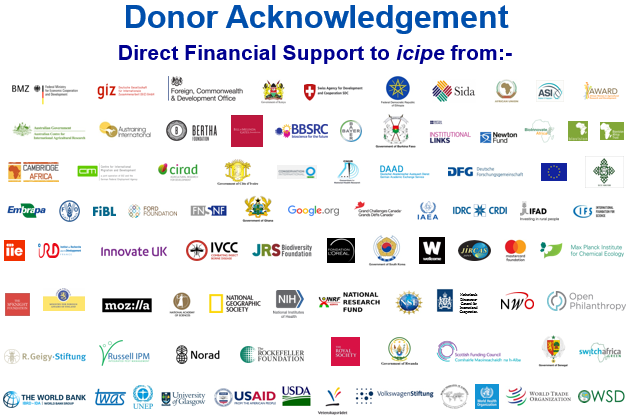
\includegraphics[width=0.9\paperwidth]{figs/icipe_acknowledgement.png}};
    \end{tikzpicture}
\end{frame}

% thank you
\begin{frame}[plain]
    \begin{tikzpicture}[remember picture,overlay]
        \fill[alpha] (current page.south west) rectangle (current page.north east);
        \node[anchor=south, text width=0.8\paperwidth, align=center, font=\bfseries\Large, text=white]
        at ([yshift=1.6cm]current page.center) {\fontsize{35pt}{16.8pt}\selectfont Thank you};
        
        \node[anchor=north west, xshift=-0.14cm, yshift=-0.25\paperwidth,]
        at (current page.north west) {\centering 
\includegraphics[width=\paperwidth]{figs/icipe_bt_line.png}};

        \node[anchor=north west, xshift=0, yshift=-0.3\paperwidth,
        fill=white, minimum height=8cm, text width=\paperwidth, inner sep=5pt]
        at (current page.north west){}; 
        
        \node[anchor=south, xshift=-0.14cm, align=center] at ([yshift=-0.2cm]current page.center) {\centering 
\includegraphics[width=2.2cm]{figs/icipe_logo.png}};

        \node[anchor=south, text width=0.8\paperwidth, align=center, font=\bfseries\Large, text=black]
        at ([yshift=-0.65cm]current page.center) {\fontsize{8pt}{16.8pt}\selectfont International Centre of Insect Physiology and Ecology};

        \node[anchor=south, xshift=-0.14cm, align=center] at ([yshift=-3.7cm]current page.center) {
            \begin{minipage}{0.48\textwidth}
                \fontsize{7pt}{16.8pt}\selectfont
                P.O. Box 30772-00100, Nairobi, Kenya \\
                Tel: +254 (20) 8632000 \\
                E-mail: {\color{alpha}\url{icipe@icipe.org}} \\
                Website: {\color{alpha} \url{www.icipe.org}} \\
                Support icipe: {\color{alpha} \url{www.icipe.org/support-icipe}}
            \end{minipage}
            \hfill
            \begin{minipage}{0.48\textwidth}
                \fontsize{7pt}{16.8pt}\selectfont
                \color{alpha}\faFacebook \quad \url{facebook.com/icipe.insects/icipe} \\
                \color{alpha} \faTwitter \quad \url{twitter.com/icipe} \\
                \color{alpha} \faLinkedin \quad \url{linkedin.com/company/icipe}
            \end{minipage}
        };
    \end{tikzpicture}
\end{frame}

\end{document}